% Options for packages loaded elsewhere
\PassOptionsToPackage{unicode}{hyperref}
\PassOptionsToPackage{hyphens}{url}
\PassOptionsToPackage{dvipsnames,svgnames,x11names}{xcolor}
%
\documentclass[
  12pt,
]{article}
\usepackage{amsmath,amssymb}
\usepackage{iftex}
\ifPDFTeX
  \usepackage[T1]{fontenc}
  \usepackage[utf8]{inputenc}
  \usepackage{textcomp} % provide euro and other symbols
\else % if luatex or xetex
  \usepackage{unicode-math} % this also loads fontspec
  \defaultfontfeatures{Scale=MatchLowercase}
  \defaultfontfeatures[\rmfamily]{Ligatures=TeX,Scale=1}
\fi
\usepackage{lmodern}
\ifPDFTeX\else
  % xetex/luatex font selection
\fi
% Use upquote if available, for straight quotes in verbatim environments
\IfFileExists{upquote.sty}{\usepackage{upquote}}{}
\IfFileExists{microtype.sty}{% use microtype if available
  \usepackage[]{microtype}
  \UseMicrotypeSet[protrusion]{basicmath} % disable protrusion for tt fonts
}{}
\makeatletter
\@ifundefined{KOMAClassName}{% if non-KOMA class
  \IfFileExists{parskip.sty}{%
    \usepackage{parskip}
  }{% else
    \setlength{\parindent}{0pt}
    \setlength{\parskip}{6pt plus 2pt minus 1pt}}
}{% if KOMA class
  \KOMAoptions{parskip=half}}
\makeatother
\usepackage{xcolor}
\usepackage[margin=1in]{geometry}
\usepackage{graphicx}
\makeatletter
\def\maxwidth{\ifdim\Gin@nat@width>\linewidth\linewidth\else\Gin@nat@width\fi}
\def\maxheight{\ifdim\Gin@nat@height>\textheight\textheight\else\Gin@nat@height\fi}
\makeatother
% Scale images if necessary, so that they will not overflow the page
% margins by default, and it is still possible to overwrite the defaults
% using explicit options in \includegraphics[width, height, ...]{}
\setkeys{Gin}{width=\maxwidth,height=\maxheight,keepaspectratio}
% Set default figure placement to htbp
\makeatletter
\def\fps@figure{htbp}
\makeatother
\setlength{\emergencystretch}{3em} % prevent overfull lines
\providecommand{\tightlist}{%
  \setlength{\itemsep}{0pt}\setlength{\parskip}{0pt}}
\setcounter{secnumdepth}{5}
\newlength{\cslhangindent}
\setlength{\cslhangindent}{1.5em}
\newlength{\csllabelwidth}
\setlength{\csllabelwidth}{3em}
\newlength{\cslentryspacingunit} % times entry-spacing
\setlength{\cslentryspacingunit}{\parskip}
\newenvironment{CSLReferences}[2] % #1 hanging-ident, #2 entry spacing
 {% don't indent paragraphs
  \setlength{\parindent}{0pt}
  % turn on hanging indent if param 1 is 1
  \ifodd #1
  \let\oldpar\par
  \def\par{\hangindent=\cslhangindent\oldpar}
  \fi
  % set entry spacing
  \setlength{\parskip}{#2\cslentryspacingunit}
 }%
 {}
\usepackage{calc}
\newcommand{\CSLBlock}[1]{#1\hfill\break}
\newcommand{\CSLLeftMargin}[1]{\parbox[t]{\csllabelwidth}{#1}}
\newcommand{\CSLRightInline}[1]{\parbox[t]{\linewidth - \csllabelwidth}{#1}\break}
\newcommand{\CSLIndent}[1]{\hspace{\cslhangindent}#1}
\ifLuaTeX
\usepackage[bidi=basic]{babel}
\else
\usepackage[bidi=default]{babel}
\fi
\babelprovide[main,import]{spanish}
% get rid of language-specific shorthands (see #6817):
\let\LanguageShortHands\languageshorthands
\def\languageshorthands#1{}
\ifLuaTeX
  \usepackage{selnolig}  % disable illegal ligatures
\fi
\IfFileExists{bookmark.sty}{\usepackage{bookmark}}{\usepackage{hyperref}}
\IfFileExists{xurl.sty}{\usepackage{xurl}}{} % add URL line breaks if available
\urlstyle{same}
\hypersetup{
  pdftitle={Incurred But Not Reported (IBNR)},
  pdfauthor={Ignacio Campón \& Joaquín Viola},
  pdflang={es},
  colorlinks=true,
  linkcolor={blue},
  filecolor={Maroon},
  citecolor={blue},
  urlcolor={blue},
  pdfcreator={LaTeX via pandoc}}

\title{Incurred But Not Reported (IBNR)}
\usepackage{etoolbox}
\makeatletter
\providecommand{\subtitle}[1]{% add subtitle to \maketitle
  \apptocmd{\@title}{\par {\large #1 \par}}{}{}
}
\makeatother
\subtitle{Seguros Generales y Modelos de Riesgo}
\author{Ignacio Campón \& Joaquín Viola}
\date{}

\begin{document}
\maketitle

\maketitle

\thispagestyle{empty} % Hide header and footer on the title page
\vspace*{\fill} % Pushes content to the bottom of the page
\begin{center}

\includegraphics[width=16cm]{imagenes/logo_inst_80.png}\\[1cm] % Adjust image placement
\end{center}

\newpage

\tableofcontents

\newpage

\hypertarget{introducciuxf3n}{%
\section{Introducción}\label{introducciuxf3n}}

En este trabajo se pretende abordar distintos métodos para el cálculo de
reservas técnicas asociadas al IBNR. El IBNR por sus siglas en inglés,
son los siniestros incurridos y que aún no fueron reclamados. En muchos
países, los seguros de responsabilidad civil, cuentan con un período de
10 años para el reclamo de un seguro luego de que el siniestro haya
ocurrido.

La idea principal de las reservas de IBNR es poder estar cubierto en el
futuro de siniestros que ocurrieron en el año corriente (mientras está
activa la poliza), pero el reclamo es efectuado en los años siguientes.

Para poder calcular las reservas de IBNR hay varios métodos, basados en
la utilización de información previa (recolectada en años anteriores),
para poder predecir cómo se comportan los reclamos en los años
siguientes.

Se suele trabajar con 3 matrices triangulares, donde las filas son años,
y las columnas son los años transcurridos. Observesé el cuadro
\ref{tabla1}, en la última fila se encuentra el último año, el cuál se
tiene datos para una sola columna, el año corriente. La fila anterior
tendrá una columna más, es decir tendrá información de dos períodos
transcurridos, de esta manera se llega a la primer fila, la cuál es el
último año que se tiene en cuenta, y para el cual se tiene información
de todos los años transcurridos, de esta manera queda explicada la forma
de la matriz triangular.

\begin{table}[ht]
\centering
\begingroup\fontsize{8.5pt}{10pt}\selectfont
\begin{tabular}{ccccccccccc}
  \hline
 & 1 & 2 & 3 & 4 & 5 & 6 & 7 & 8 & 9 & 10 \\ 
  \hline
1999 & 652799 & 1383776 & 2634200 & 3167840 & 3842289 & 4029679 & 4454460 & 4817622 & 5012751 & 5099688 \\ 
  2000 & 1360795 & 2480988 & 2806387 & 3592401 & 3451088 & 3931688 & 4491687 & 4165270 & 4221137 &  \\ 
  2001 & 1985553 & 3275646 & 3290023 & 3945474 & 4961886 & 4975029 & 5914580 & 5969088 &  &  \\ 
  2002 & 2901555 & 4528347 & 4556763 & 5790821 & 6444829 & 7957380 & 8581805 &  &  &  \\ 
  2003 & 3572829 & 4717083 & 5937065 & 6835232 & 7309686 & 7276239 &  &  &  &  \\ 
  2004 & 2578343 & 4423917 & 4664371 & 5348014 & 5882585 &  &  &  &  &  \\ 
  2005 & 4051902 & 6081465 & 8618348 & 9901076 &  &  &  &  &  &  \\ 
  2006 & 5030173 & 8881224 & 12548654 &  &  &  &  &  &  &  \\ 
  2007 & 6849422 & 9171465 &  &  &  &  &  &  &  &  \\ 
  2008 & 10120889 &  &  &  &  &  &  &  &  &  \\ 
   \hline
\end{tabular}
\endgroup
\caption{Siniestros incurridos acumulados por año y por período transcurrido en pesos.} 
\label{tabla1}
\end{table}

La primer matriz triangular tiene la información de los pagos acumulados
de los siniestros ocurridos en cada año, y cuando fueron pagados
efectivamente. Para la primer fila, en la primer columna se tienen los
pagos de los siniestros ocurridos y pagados hace 10 años, luego en la
siguiente columna se tiene los siniestros ocurridos en ese año pero
reclamados y pagados en el siguiente, más los de la columna anterior
(por ser pagos acumulados) y así sucesivamente.

La segunda matriz es la matriz de siniestros pendientes de pagos, que
tiene para cada celda (año), los siniestros ocurridos en la fila a la
que pertenece, y reportados pasado los años según la columna en la que
está, es decir, salvo los de la primera columna, todos son reportados
luego de pasado cierta cantidad de años, pero que aún no han sido
pagados, ya sea por litigio, o por que se está estimando el valor final
a pagar.

En última instancia tenemos la matriz triangular de siniestros
incurridos (cuadro \ref{tabla1}). En cada celda se tiene la suma de las
dos matrices anteriores que es el total de los siniestros acumulados y
reservados ocurridos en cada año y que han ido ocurriendo a lo largo de
los años siguientes. Cada diagonal (en el sentido inverso,
\(X_{1,n}, X_{2,n-1}, \ldots , X_{n,1}\)) corresponde a los pagos
acumulados y reservados de un ejercicio contable.

La reserva de IBNR es la reserva que debe tener la compañía pasado \(n\)
años (en general 10 años) para poder cubrir los siniestros ocurridos en
el año actual, y que serán reportados durante los siguientes años.

Se trabajará con la matriz de siniestros trabajada en el curso de
``Solvencias de Compañías Aseguradoras'' brindado por el profesor
\textit{Enrique Arónica} en Noviembre de 2023 en la Facultad de Ciencias
Económicas (UDELAR). Se cuenta con la matriz de pagos acumulados, la
matriz de siniestros pendientes de pagos y la de siniestros incurridos.

La figura \ref{triangle} fue realizada con la función \texttt{plot} de
\texttt{R} base, la cual fue aplicada a un objeto (matriz de siniestros
incrurridos) de clase \texttt{triangle}. Esta figura nos permite ver
como crecen los siniestros incurridos en cada período con el correr de
los años, obteniendo así una línea para cada año de ocurrencia y
observando el crecimiento de los siniestros incurridos durante los
períodos de desarrollo. Cada línea representa los siniestros incurridos
en un período, y se ve como va aumentando los pagos acumulados y
reservados con el correr de los períodos.

\begin{figure}
\centering
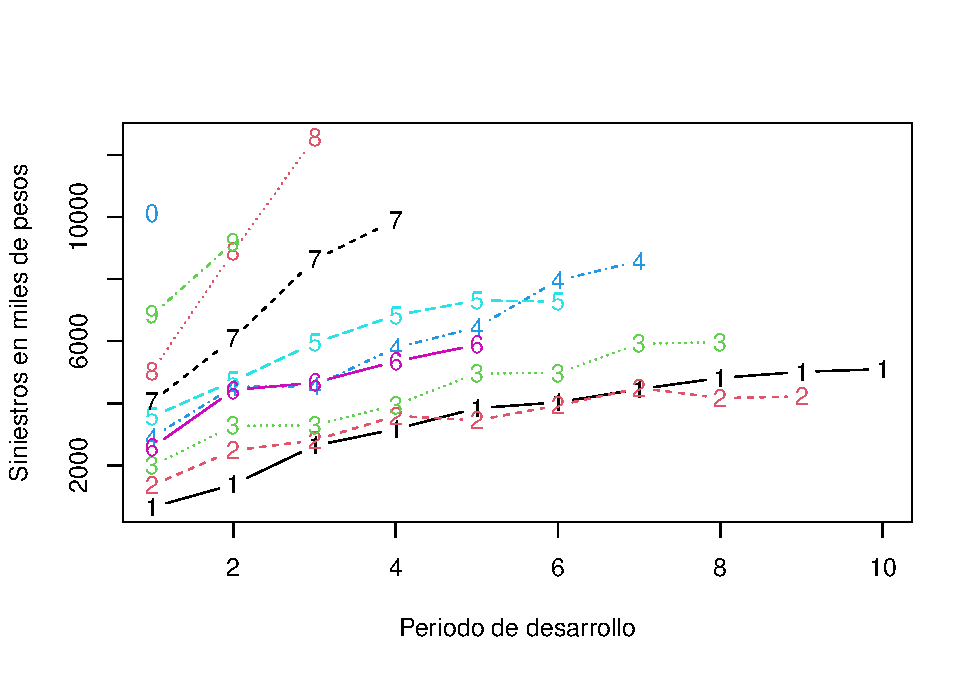
\includegraphics{informe_files/figure-latex/unnamed-chunk-4-1.pdf}
\caption{\label{triangle} Desarrollo de los reclamos por año y período.}
\end{figure}

\hypertarget{chain-ladder}{%
\section{Chain-Ladder}\label{chain-ladder}}

\hypertarget{chain-ladder-cluxe1sico}{%
\subsection{Chain Ladder `clásico'}\label{chain-ladder-cluxe1sico}}

Uno de los métodos más utilizados es el de `Chain Ladder' (Escalera de
Cadena), que a partir de la última matriz presentada en la sección
anterior calcula los factores de desarrollo, que miden el crecimiento de
los gastos por siniestro pasado los años. El factor de desarrollo
representa la proporción que aumentan el monto de los siniestros
incurridos entre dos períodos consecutivos (el factor de desarrollo
\(q_j\) representa el aumento de los siniestros incurridos entre el
período \(j\) y el \(j+1\)). Para el cálculo de este, se suma todos los
siniestros incurridos en el período \(j+1\), es decir
\(\sum_{i=1}^{n-j} X_{i,j+1}\) y se los divide entre la misma cantidad
de filas, del período anterior (\(j\)), es decir
\(\sum_{i=1}^{n-j} X_{i,j}\)

\[
\hat{q}_{j} = \frac{\sum_{i=1}^{n-j} X_{i,j+1}}{\sum_{i=1}^{n-j} X_{i,j}}
\]

\begin{figure}
\centering
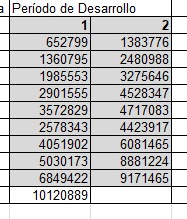
\includegraphics{imagenes/captura1.jpg}
\caption{En gris, las filas de la columna del período 2 y período 1 que
se dividen para calcular el factor de desarrollo del período 1}
\end{figure}

El total a pagar y reservar por los siniestros ocurridos en el año \(i\)
es el producto de \(X_i = Q_j\cdot X_{i,j}\), donde \(Q_j\) es el factor
de desarrollo acumulado, que representa el aumento de los siniestros
pagados acumulados y reservados al período \(j\) (\(X_{i,j}\)), hasta el
total que se va a pagar por los siniestros incurridos en el año \(i\)
(\(X_i\)). Se puede demostrar que el factor de desarrollo acumulado se
calcula de forma iterativa a través de la fórmula
\(Q_{j-1}=q_{j-1}\cdot Q_{j}\), y en particular, \(Q_n = 1\) que
representa el aumento de los siniestros pagados acumulados y reservados
ocurridos en el primer año que se está tomando, y acumulado durante los
\(n\) años siguientes, que luego, por cuestiones jurídicas no habrá
nuevos reclamos.

Luego, podemos decir que \(X_i\) es la pérdida esperada por los
siniestros incurridos en el año i, y nuestra reserva de \(IBNR_i\), que
es la reserva para los siniestros ocurridos en el año \(i\) y que fueron
denunciados en los años posteriores será la diferencia entre la pérdida
esperada, y el último período para el que tenemos los pagos acumulados y
reservados en la matriz de siniestros incurridos (\(X_{i,n-i+1}\))

\begin{verbatim}
##       Incurridos_Acumulados QAcum Perdida_Esperada Reserva_IBNR
## 1999                5099688 1.000          5099688         0.00
## 2000                4221137 1.017          4292896     71759.33
## 2001                5969088 1.045          6237697    268608.96
## 2002                8581805 1.052          9028059    446253.86
## 2003                7276239 1.180          8585962   1309723.02
## 2004                5882585 1.278          7517944   1635358.63
## 2005                9901076 1.421         14069429   4168353.00
## 2006               12548654 1.687         21169579   8620925.30
## 2007                9171465 2.125         19489363  10317898.12
## 2008               10120889 3.297         33368571  23247682.03
## Total              78772626    NA        128859188  50086562.25
\end{verbatim}

También se puede asignar un valor mayor a 1 para el factor de desarrollo
del último año \(Q_n>1\), por distintas cuestiones que no son de
particular interés en este trabajo, por ejemplo \(Q_n=1,05\), y luego
los siguientes factores de desarrollo quedaran determinados a partir de
este primero.

\hypertarget{chain-ladder-con-regresiuxf3n}{%
\subsection{Chain Ladder con
regresión}\label{chain-ladder-con-regresiuxf3n}}

Este modelo permite calcular el factor de desarrollo para \(Q_n\)
asumiendo una estructura de regresión para los factores de desarrollos
(simples) en función de los períodos de desarrollo. Si bien estos no
varían mucho a lo largo del tiempo, si se puede observar una estructura
de regresión lineal si hacemos el logaritmo del aumento proporcional
(\(q-1\)) de los siniestros incurridos en función de los períodos de
desarrollo \(L(q-1) \sim \text{períodos de desarrollo}\).

\[
L(q_j -1) = \alpha + \beta\times j
\]

\begin{verbatim}
## [1] 1.550679 1.259512 1.186842 1.112016 1.083055 1.121986 1.006141 1.027942
## [9] 1.017343
\end{verbatim}

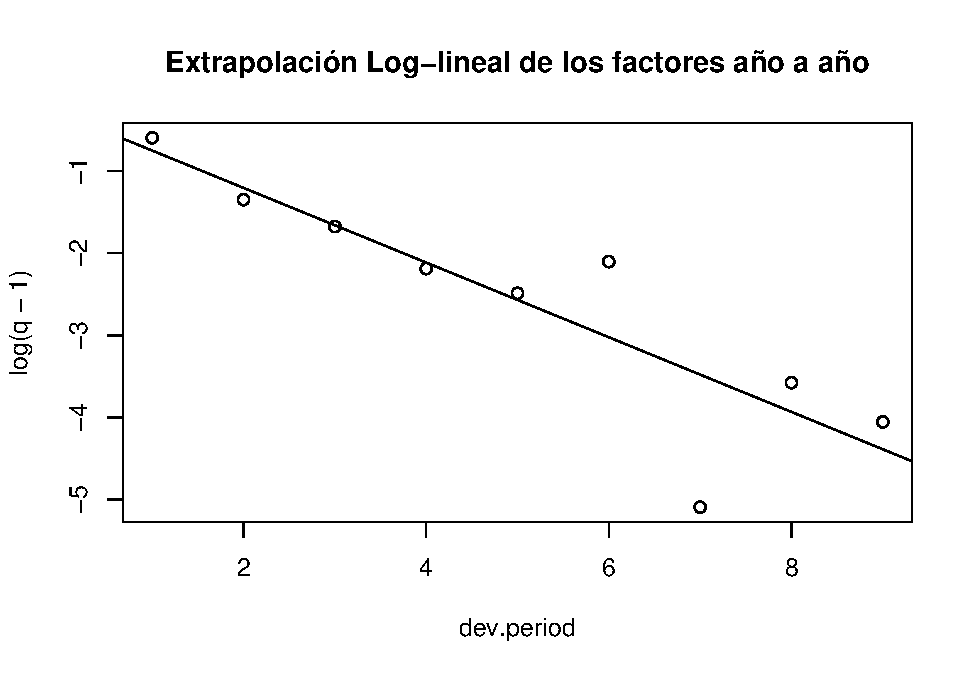
\includegraphics{informe_files/figure-latex/unnamed-chunk-7-1.pdf}

\begin{verbatim}
## integer(0)
\end{verbatim}

Para esto es necesario haber calculado los factores de desarrollo simple
y hacer el modelo correspondiente, previamente chequendo si para el
gráfico de dispersión de los datos corresopnde el modelo de regresión
lineal. Luego, se sugiere extrapolar los datos para 100 períodos de
desarrollo, y se puede observar que se empieza a estabilizar
\(L(q_j -1)\) cuando \(j\) aumenta, y si tomamos \(Q_n\) el factor de
desarrollo acumulado para el período que estamos trabajando, podemos
calcular \(\hat{Q_n} = \prod_{j\geq n} \hat{q_{j}} = 1.021795\).

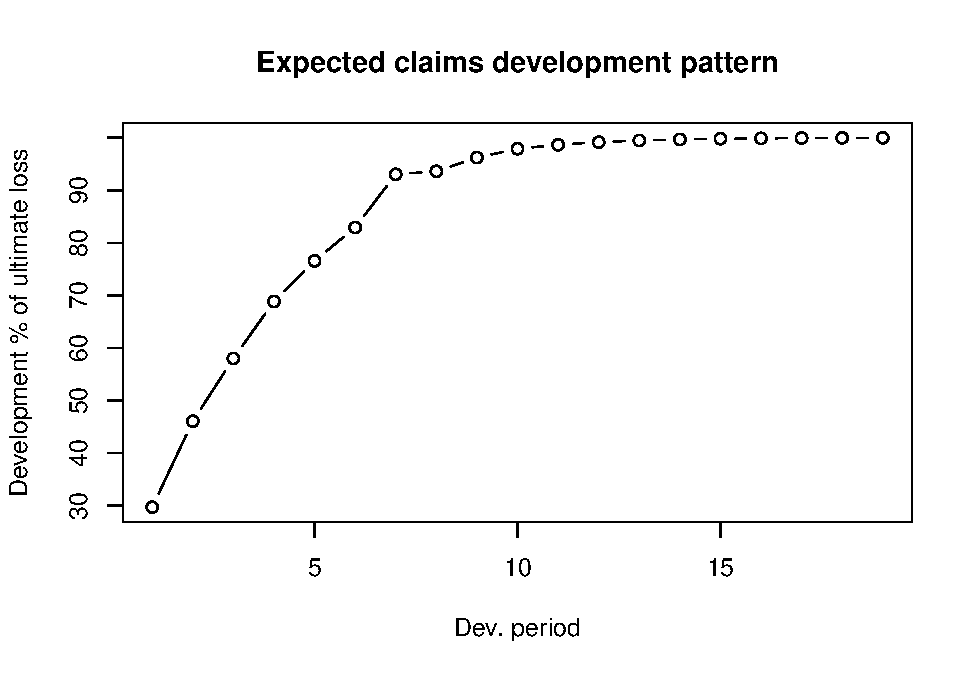
\includegraphics{informe_files/figure-latex/unnamed-chunk-8-1.pdf}
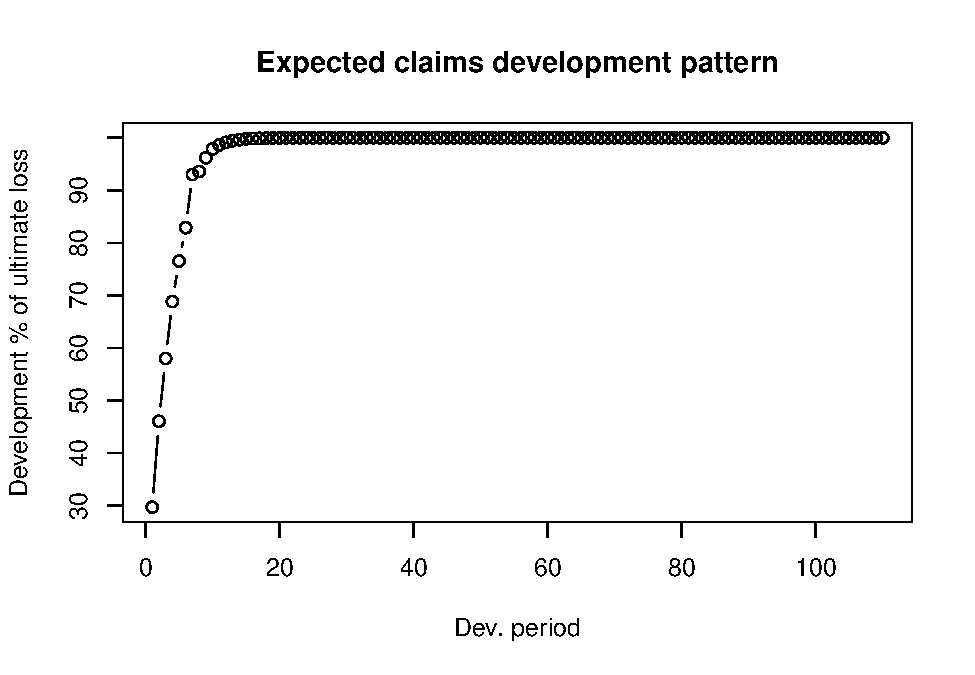
\includegraphics{informe_files/figure-latex/unnamed-chunk-8-2.pdf}

\begin{verbatim}
## [1] 1.021795
\end{verbatim}

Nuestros factores de desarrollo serán los obtenidos normalmente hasta el
momento \(n-1=9\) y para \(q_n=q_{10}\) se le asigna el valor de
\(\hat{Q_n}\) calculado que ya se mostró que para el último período de
desarrollo era válida la equivalencia.

\begin{verbatim}
##       Incurridos_Acumulados2    Qs Perdida_Esperada2 Reserva_IBNR2
## 1999                 5099688 1.022           5211881      112193.1
## 2000                 4221137 1.040           4389982      168845.5
## 2001                 5969088 1.069           6380955      411867.1
## 2002                 8581805 1.075           9225440      643635.4
## 2003                 7276239 1.206           8775144     1498905.2
## 2004                 5882585 1.306           7682656     1800071.0
## 2005                 9901076 1.453          14386263     4485187.4
## 2006                12548654 1.724          21633879     9085225.5
## 2007                 9171465 2.172          19920422    10748957.0
## 2008                10120889 3.368          34087154    23966265.2
## Total               78772626    NA         131693778    52921152.4
\end{verbatim}

Se observa que al asignarle un factor de desarrollo acumulado mayor a 1
para el último período de desarrollo se obtiene que las reservas por
IBNR aumentan aproximadamente en \$3.000.000 respecto al método clásico,
que representa aproximadamente un aumento del \%5.

\hypertarget{mack-chain-ladder}{%
\section{Mack Chain-Ladder}\label{mack-chain-ladder}}

Thomas Mack publica en 1993 un método para obtener estimaciones de los
errores estándar de las estimaciones de pérdida esperada, y por
consecuencia del IBNR, se basa en la matriz triangular de pérdida
agregada pero nosotros lo usaremos sobre la matriz triangular de
siniestros incurridos, y se puede predecir el triángulo inferior
faltante de la matriz, es decir, los siniestros incurridos a futuro de
cada año para cada período de desarrollo.

Para predecir los siniestros incurridos a futuro \(X_{i,j}\) con
\(j>n-i+1\) se asume:

\begin{itemize}

\item $\mathbb{E}(q_{i,j}|X_{i,1},\ldots,X_{i,j}) = q_j$ con $q_{i,j} = \frac{X_{i,j+1}}{X_{i,j}}$

\item $\mathbb{V}(q_{i.j}|X_{i,1},\ldots,X_{i,j}) = \frac{\sigma^2_j}{w_{i,j}X_{i,j}^\alpha} $

\item $\{ X_{i,1},\ldots,X_{i,n} \}, \{X_{k,1},\ldots,X_{k,n}\}$ son independientes del período de origen ($i \neq k$)

\end{itemize}

Con \(w_{i,j} \in [0;1]\) y \(\alpha \in \{0,1,2\}\), se obtienen
estimaciones insesgadas de las pérdidas esperadas y de las reservas de
IBNR junto a los errores estándar y el coeficiente de variación.

Luego, a partir de la fórmula del error cuadrático medio,
\(ECM(\hat{X}_{i,n})=\mathbb{E}((\hat{X}_{i,n}-X_{i,n})^2|X_{i,1}\ldots,X_{i,n-i+1})=\mathbb{V}(\hat{X}_{i,n}) + (\mathbb{E}(X_{i,n}|X_{i,1}\ldots,X_{i,n-i+1})-\hat{X}_{i,n})^2\)
se podrá calcular el error cuadrático medio como la suma de los errores
estocásticos y el error de estimación y se necesitará una fórmula para
la varianza.

Se puede notar que el factor de desarrollo \(q_j\) es el promedio
ponderado de los factores \(q_{i,j}=X_{i,j+1}/X_{i,j}\), por lo que la
varianza de \(X_{i,j+1}/X_{i,j}\) (dado los siniestros hasta el período
de desarrollo j) es inversamente proporcional a \(X_{i,j}\), donde se
asume que todos los siniestros incurridos pesan igual y \(\alpha=1\) en
las condiciones planteadas anteriormente.

\[
\mathbb{V}(X_{i,j+1}|X_{i,1},\ldots,X_{i,j}) = X_{i,j}\cdot \sigma_j^2
\] Donde \(\sigma_j^2\) es un parámetro desconocido que debe ser
estimado, y es la varianza implícita bajo el método de `Chain Ladder'.
Por lo que la varianza estimada será la suma de los errores al cuadrado
ponderados de la estimación de los factores de desarrollo año a año.

\[
\hat{\sigma_j}^2 = \frac{1}{n-j-1}\cdot \sum_{i=1}^{n-j} X_{i,j}\left( \frac{X_{i,j+1}}{X_{i,j}} - \hat{q_j} \right)^2=\frac{1}{n-j-1}\cdot \sum_{i=1}^{n-j} X_{i,j}\left( q_{i,j} - \hat{q_j} \right)^2
\]

Siendo \(\hat{\sigma_j}^2\) un estimador insesgado para
\(1 \leq j \leq n-2\), obteniendo una estimación del desvío al hacer la
raíz. Para estimar \(\sigma_{n-1}\) , si se tiene que
\(\hat{q}_{n-1}=1\) se puede utilizar \(\sigma_{n-1}=0\) ya que se asume
que el desarrollo de los siniestros termina en el tiempo \(n-1\), de lo
contrario se puede extrapolar utilizando la reducción exponencial de los
desvíos de forma tal que \(\hat{\sigma}_{n-1}\) cumpla con la razón.

\[
\frac{\hat{\sigma}_{n-3}}{\hat{\sigma}_{n-2}} = \frac{\hat{\sigma}_{n-2}}{\hat{\sigma}_{n-1}}
\]

\[
\hat{\sigma}_{n-1} = \frac{\hat{\sigma}_{n-2}^2}{\hat{\sigma}_{n-3}}
\]

Siendo \(R_i\) las reservas de IBNR del año \(i\), estas son calculadas
como \(R_i = X_{i,n} - X_{i,n-i+1}\) y estimadas de la forma
\(\hat{R}_i = \hat{X}_{i,n} - X_{i,n-i+1}\) donde el total de los costos
incurridos del año \(i\) son estimados a través de los factores de
desarrollo, ya sea calculando el total para todos los años de desarrollo
con los factores año a año, o a través del factor de desarrollo
acumulado \(\hat{X}_{i,n} = Q_{n-i+1}\cdot X_{i,n-i+1}\). Luego, como la
única parte aleatoria de \(\hat{R}_i\) es \(\hat{X}_{i,n}\) el
\(ECM(\hat{R}_i) = ECM(\hat{X}_{i,n})\)

\[
\widehat{ECM}(\hat{R}_i) = \hat{X}_{i,n}^2 \sum_{j=n-i+1}^{n-1} \frac{\hat{\sigma_j}^2}{\hat{q}_j}\left( \frac{1}{\hat{X}_{i,j}} - \frac{1}{\sum_{l=1}^{I-j}X_{l,j}} \right)
\]

La función `MackChainLadder' del paquete `ChainLadder' nos da una tabla
con las reservas de IBNR para cada año, su desvío y su coeficiente de
variación, y las mismas medidas para el total, teniendo especial
atentción de que el desvío del total no es igual a la suma del desvío,
nos muestra la última pérdida obtenida, la última pérdida esperada, la
relación entre estas, la reserva de IBNR, el desvío y el coeficiente de
variación.

\begin{verbatim}
## MackChainLadder(Triangle = tri)
## 
##          Latest Dev.To.Date   Ultimate       IBNR  Mack.S.E CV(IBNR)
## 1999  5,099,688       1.000  5,099,688          0         0      NaN
## 2000  4,221,137       0.983  4,294,345     73,208   158,102    2.160
## 2001  5,969,088       0.956  6,242,289    273,201   246,430    0.902
## 2002  8,581,805       0.950  9,029,697    447,892   708,613    1.582
## 2003  7,276,239       0.847  8,589,919  1,313,680   782,964    0.596
## 2004  5,882,585       0.782  7,521,436  1,638,851 1,070,034    0.653
## 2005  9,901,076       0.703 14,077,509  4,176,433 1,880,771    0.450
## 2006 12,548,654       0.593 21,175,489  8,626,835 2,602,113    0.302
## 2007  9,171,465       0.471 19,492,933 10,321,468 3,717,510    0.360
## 2008 10,120,889       0.303 33,356,395 23,235,506 6,120,205    0.263
## 
##                   Totals
## Latest:    78,772,626.00
## Dev:                0.61
## Ultimate: 128,879,702.24
## IBNR:      50,107,076.24
## Mack.S.E   11,156,939.54
## CV(IBNR):           0.22
\end{verbatim}

También se puede acceder a los factores mediante acciedendo a
`mackTRI\$f', o a la matriz completa con la estimación de los siniestros
incurridos en los años siguientes mediante `mackTRI\$FullTriangle'.

\begin{verbatim}
##  [1] 1.550679 1.259512 1.186842 1.112016 1.083055 1.121986 1.006141 1.027942
##  [9] 1.017343 1.000000
\end{verbatim}

\begin{verbatim}
##       dev
## origin        1        2        3        4        5        6        7        8
##   1999   652799  1383776  2634200  3167840  3842289  4029679  4454460  4817622
##   2000  1360795  2480988  2806387  3592401  3451088  3931688  4491687  4165270
##   2001  1985553  3275646  3290023  3945474  4961886  4975029  5914580  5969088
##   2002  2901555  4528347  4556763  5790821  6444829  7957380  8581805  8634502
##   2003  3572829  4717083  5937065  6835232  7309686  7276239  8163841  8213971
##   2004  2578343  4423917  4664371  5348014  5882585  6371162  7148357  7192252
##   2005  4051902  6081465  8618348  9901076 11010150 11924596 13379234 13461390
##   2006  5030173  8881224 12548654 14893269 16561547 17937063 20125140 20248719
##   2007  6849422  9171465 11551567 13709884 15245604 16511825 18526042 18639802
##   2008 10120889 15694252 19767093 23460415 26088346 28255109 31701847 31896514
##       dev
## origin        9       10
##   1999  5012751  5099688
##   2000  4221137  4294345
##   2001  6135874  6242289
##   2002  8875763  9029697
##   2003  8443483  8589919
##   2004  7393214  7521436
##   2005 13837522 14077509
##   2006 20814500 21175489
##   2007 19160627 19492933
##   2008 32787752 33356395
\end{verbatim}

Y al resumen final separado por año o para el total se accede mediante
summary de la manera:

\begin{verbatim}
##        Latest Dev.To.Date Ultimate       IBNR  Mack.S.E  CV(IBNR)
## 1999  5099688   1.0000000  5099688        0.0       0.0       NaN
## 2000  4221137   0.9829525  4294345    73207.9  158102.2 2.1596328
## 2001  5969088   0.9562338  6242289   273201.1  246430.1 0.9020099
## 2002  8581805   0.9503979  9029697   447892.3  708612.6 1.5821048
## 2003  7276239   0.8470672  8589919  1313680.4  782964.5 0.5960083
## 2004  5882585   0.7821093  7521436  1638851.2 1070034.2 0.6529173
## 2005  9901076   0.7033259 14077509  4176433.0 1880770.5 0.4503294
## 2006 12548654   0.5926028 21175489  8626835.4 2602113.4 0.3016301
## 2007  9171465   0.4705020 19492933 10321468.4 3717510.0 0.3601726
## 2008 10120889   0.3034167 33356395 23235506.5 6120205.1 0.2633988
\end{verbatim}

\begin{verbatim}
##                  Totals
## Latest:    7.877263e+07
## Dev:       6.112105e-01
## Ultimate:  1.288797e+08
## IBNR:      5.010708e+07
## Mack S.E.: 1.115694e+07
## CV(IBNR):  2.226620e-01
\end{verbatim}

Y se accede a distintos gráficos con la función plot

\begin{figure}
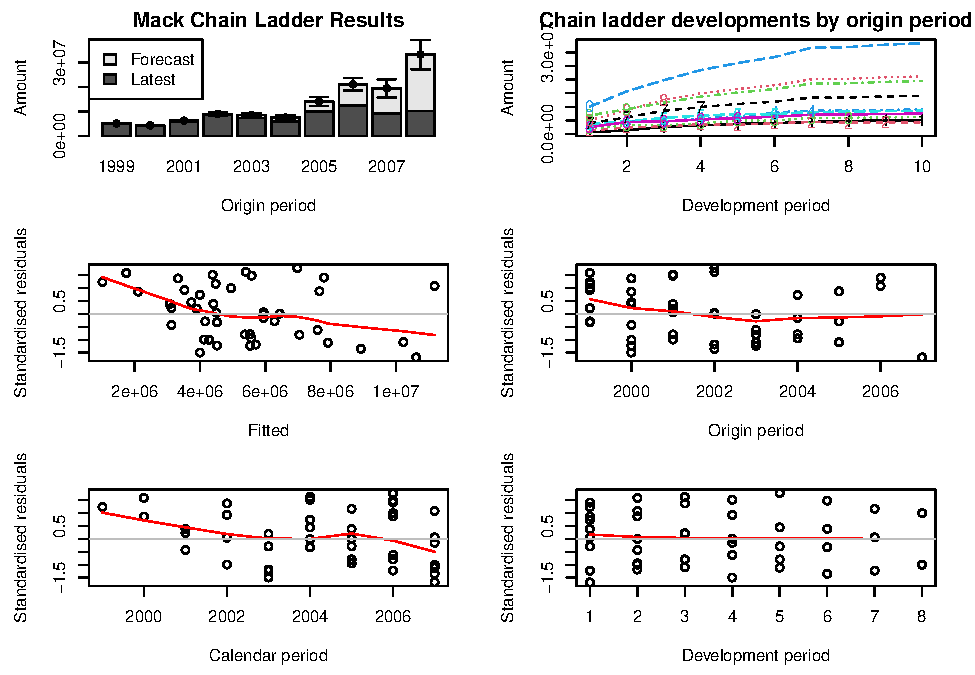
\includegraphics[width=1\linewidth]{informe_files/figure-latex/unnamed-chunk-17-1} \end{figure}

También se puede graficar la predicción del desarrollo de los siniestros
incurridos a futuro junto a una medida de la dispersión, separado por
cada año de ocurrencia

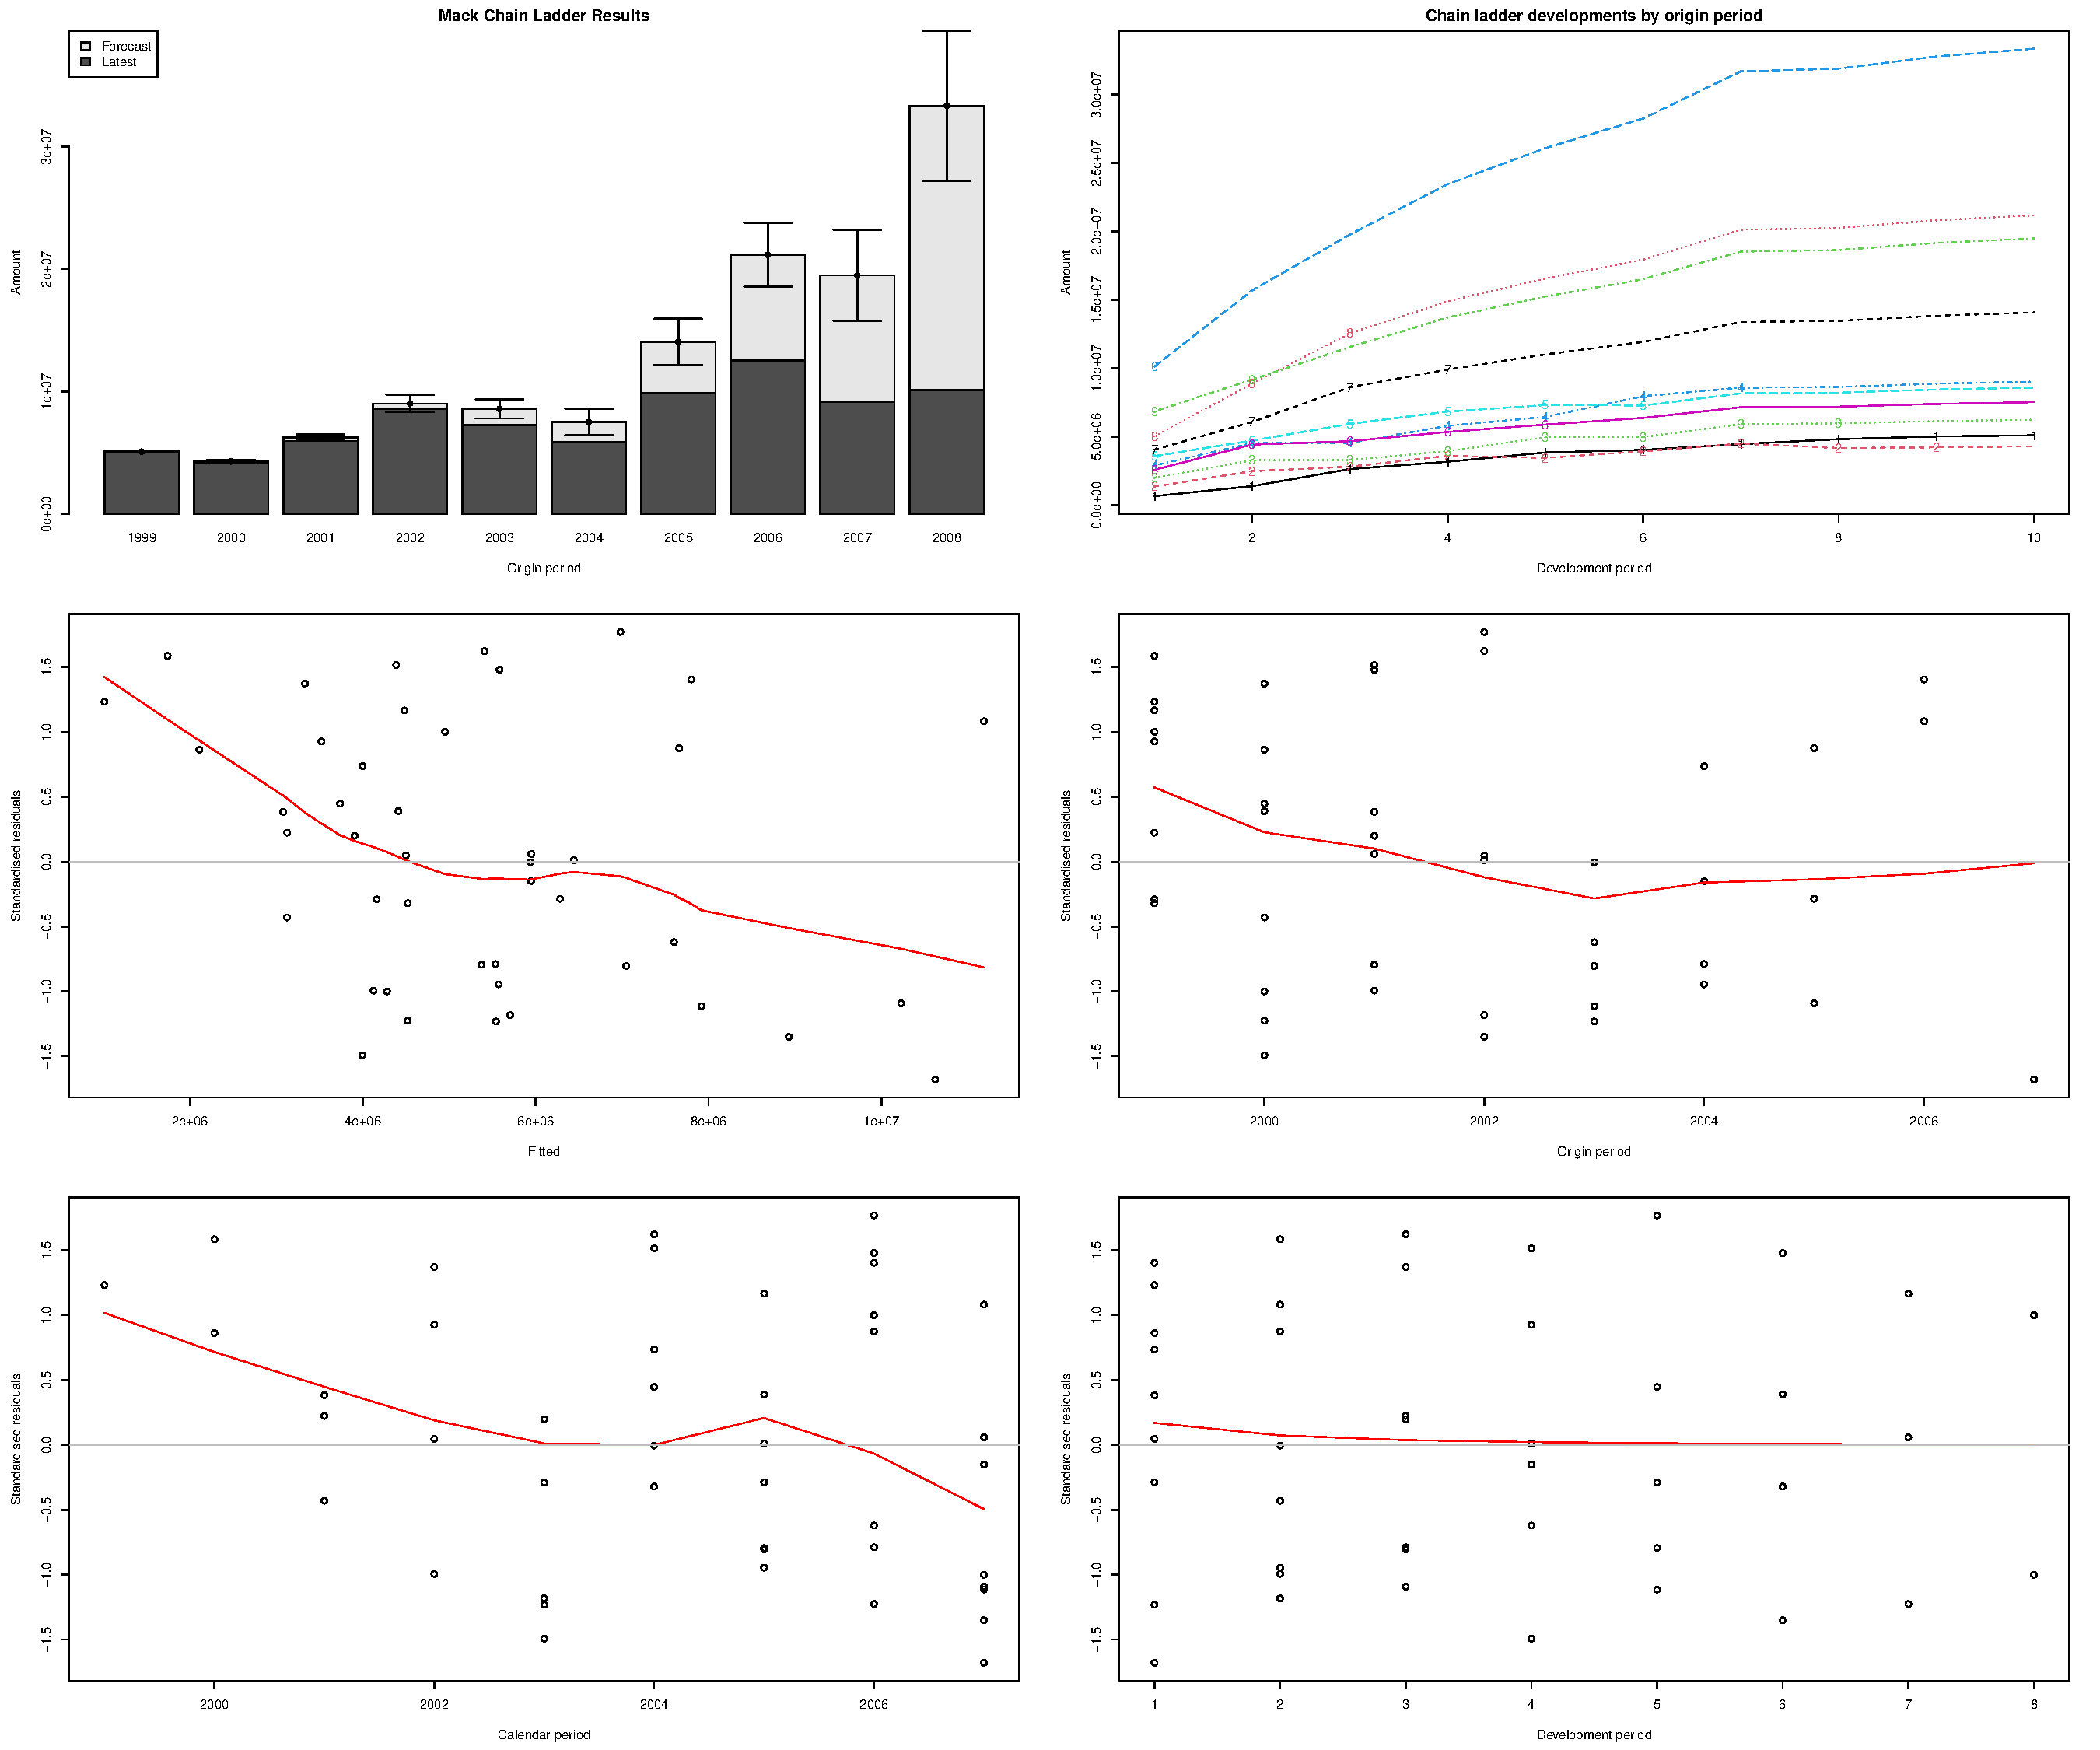
\includegraphics{informe_files/figure-latex/unnamed-chunk-18-1.pdf}

\hypertarget{munich-chain-ladder}{%
\section{Munich Chain Ladder}\label{munich-chain-ladder}}

El método de Munich utiliza la correlación positiva entre el triángulo
de siniestros incurridos y el triángulo de siniestros pagados acumulados
para proyectar los futuros pagos. Para esto es necesario agregarla
información los datos de siniestros pagos acumulados.

Llamando \emph{I} a la matriz de siniestros incurridos y \emph{P} a la
matriz de siniestros pagados, se halla la matriz \(P/I\) calculada como
la división de celda a celda de la matriz \emph{P} entre la matriz
\emph{I}, y representa la fracción de los siniestros incurridos que ya
están pago de cada año durante los períodos de desarrollo. Donde se
suele observar que a medida que hay más períodos de desarrollo la
mayoría de los siniestros han sido pagados.

\begin{table}[ht]
\centering
\begingroup\fontsize{8.5pt}{10pt}\selectfont
\begin{tabular}{ccccccccccc}
  \hline
 & 1 & 2 & 3 & 4 & 5 & 6 & 7 & 8 & 9 & 10 \\ 
  \hline
1999 & 0.5712 & 0.4191 & 0.2374 & 0.2043 & 0.2524 & 0.3934 & 0.5571 & 0.6733 & 0.8434 & 0.8644 \\ 
  2000 & 0.2671 & 0.2708 & 0.2546 & 0.2058 & 0.2168 & 0.2695 & 0.4919 & 0.7259 & 0.7843 &  \\ 
  2001 & 0.3263 & 0.3150 & 0.3936 & 0.4187 & 0.4143 & 0.4693 & 0.4024 & 0.3657 &  &  \\ 
  2002 & 0.1413 & 0.2445 & 0.3226 & 0.2988 & 0.3824 & 0.5337 & 0.5969 &  &  &  \\ 
  2003 & 0.2329 & 0.3176 & 0.2790 & 0.2980 & 0.3529 & 0.3592 &  &  &  &  \\ 
  2004 & 0.3728 & 0.3429 & 0.4024 & 0.4045 & 0.3816 &  &  &  &  &  \\ 
  2005 & 0.5250 & 0.5667 & 0.5095 & 0.4520 &  &  &  &  &  &  \\ 
  2006 & 0.4937 & 0.4846 & 0.4755 &  &  &  &  &  &  &  \\ 
  2007 & 0.4634 & 0.5191 &  &  &  &  &  &  &  &  \\ 
  2008 & 0.4818 &  &  &  &  &  &  &  &  &  \\ 
   \hline
\end{tabular}
\endgroup
\caption{Proporción de siniestros incurridos que han sido pagos en cada período de desarrollo.} 
\label{tabla2}
\end{table}

\hypertarget{problemas-del-chain-ladder-por-separado-scl}{%
\subsection{Problemas del Chain-Ladder por separado
(SCL)}\label{problemas-del-chain-ladder-por-separado-scl}}

Formalmente, se tiene que \((P/I)_{i,j} = P_{i,j}/I_{i,j}\), luego,
mediante los métodos vistos antes de Chain Ladder se puede estimar los
valores faltantes de ambas matrices con los factores de desarrollo año a
año a partir de la diagonal inversa, obteniendo el resultado de los
ratios si se hace Chain-Ladder por separado (Método SCL).

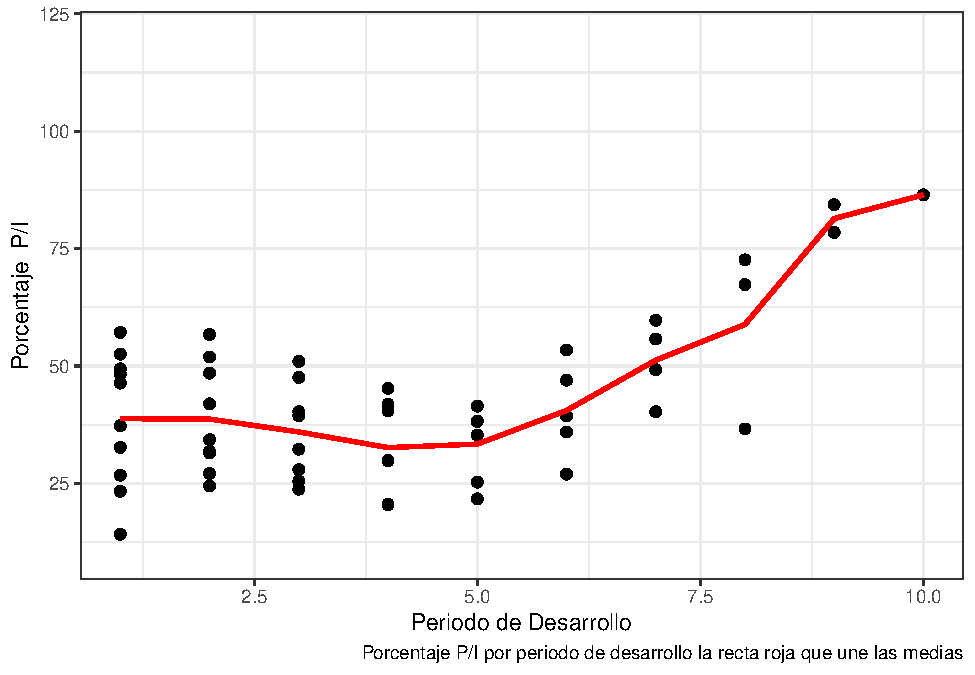
\includegraphics[width=0.5\linewidth]{informe_files/figure-latex/unnamed-chunk-22-1}
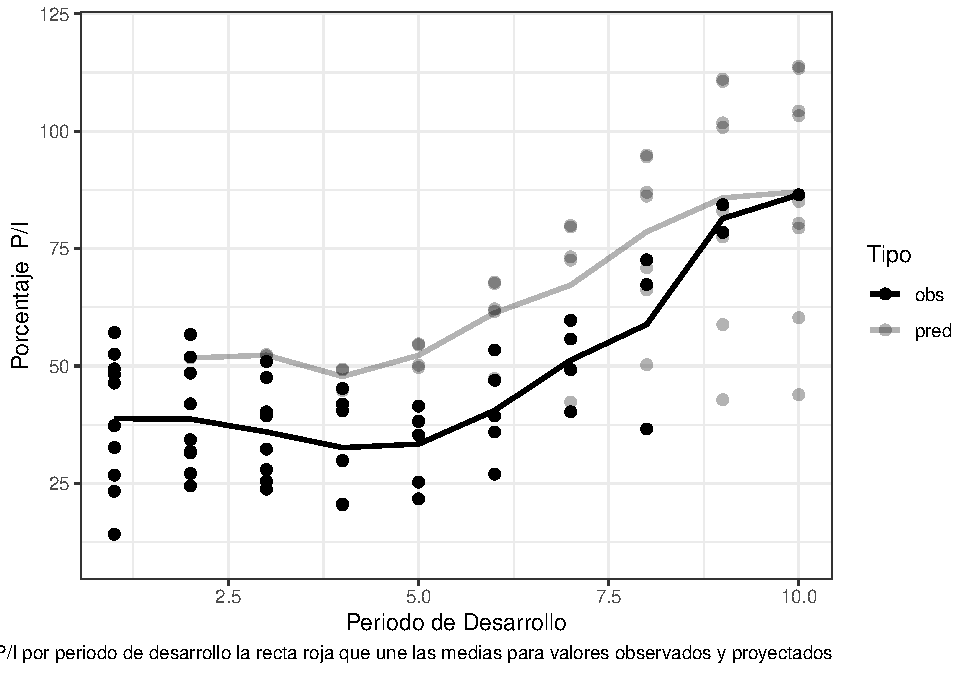
\includegraphics[width=0.5\linewidth]{informe_files/figure-latex/unnamed-chunk-22-2}
Se puede notar en la segunda figura que para los valores proyectados en
las dos matrices por separado a partir de cierto período de desarrollo
se tiene que los siniestros pagados significan una proporción mayor a 1
que los siniestros incurridos, este error se da debido a que se aplicó
el método de Chain-Ladder por separado a ambos triángulos (SCL) y no se
tuvo en cuenta la estructura de correlación entre ambos triángulos.

Para concluir el principal resultado de este método se debe hacer
cuentas con los factores de desarrollo y las proyecciones tanto en la
matriz de pagos acomulados como la de siniestros incurridos. Para esto
define el promedio de los ratios en el tiempo de desarrollo t:

\[
(P/I)_t := \frac{\sum_{j=1}^n P_{j,t}}{\sum_{j=1}^n I_{j,t}} = \frac{1}{\sum_{j=1}^n I_{j,t}}\cdot \sum_{j=1}^n I_{j,t}\cdot (P/I)_{j,t}
\]

Y luego, definiendo \(c_i:n-i+1\) como el último período de desarrollo
del que se tiene información para los siniestros, tanto los pagados
acumulados como los incurridos en el momento \(i\) y se puede observar
que los pares \((i,c_i)\) son los índices de la diagonal invertida de
las matrices. Luego, observando que para el año \(i\), los valores de
\(P_{i,t}\) y \(I_{i,t}\) son proyecciones para \(t>c_i\) se tiene que
el ratio \((P/I)_{i,t}\) se calcula

\[
(P/I)_{i,t} = \frac{P_{i,t}}{I_{i,t}} = \frac{P_{i,c_i}\cdot q_{c_i}^P \cdot \ldots \cdot q_{t-1}^P}{I_{i,c_i}\cdot q_{c_i}^I \cdot \ldots \cdot q_{t-1}^I}
\]

A partir de las fórmulas de los factores de desarrollo, se nota que para
\(t>c_i\):

\[
(P/I)_{i,t} = \frac{P_{i.c_i}\cdot \frac{\sum_{j=1}^n P_{j,t}}{\sum_{j=1}^n P_{j,c_i}}}{I_{i.c_i}\cdot \frac{\sum_{j=1}^n I_{j,t}}{\sum_{j=1}^n I_{j,c_i}}}
\] Y reordenando se tiene la siguiente relación para los ratios
proyectados mediante la aplicación de Chain-Ladder por separado:

\[
\frac{(P/I)_{i,t}}{(P/I)_t} = \frac{(P/I)_{i,c_i}}{(P/I)_{c_i}}
\]

Que indica que para cada año de accidente, el ratio de \((P/I)_{i,t}\)
con el \((P/I)_t\) promedio en el período de desarrollo t, debe cumplir
la misma relación que en el período \(c_i\), y esto se ve claramente en
el gráfico de la derecha cuando se hace Chain-Ladder por separado siendo
la principal debilidad del método.

\hypertarget{modelado-con-munich-chain-ladder}{%
\subsection{Modelado con Munich
Chain-Ladder}\label{modelado-con-munich-chain-ladder}}

Veamos que la correlación entre los factores de desarrollo para cada año
de ocurrencia del primer período de desarrollo de la matriz de pagos
acumulados, es decir, el vector de \(q_{i,1}^P\)
\(\forall i = \{1,2,\ldots,10\}\) respecto a los ratios \((P/I)_{i,1}\)
es de \(-0.7278\).

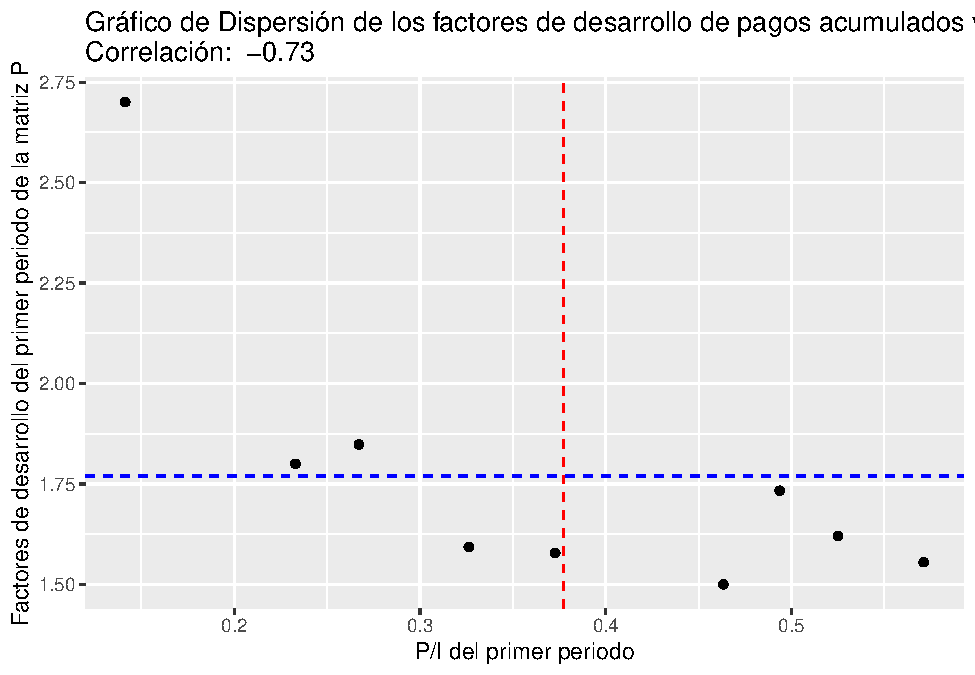
\includegraphics{informe_files/figure-latex/unnamed-chunk-24-1.pdf}

Y por otro lado, haciendo lo mismo para los factores de desarrollo
individuales del primer período de la matriz de siniestros incurridos y
los ratios del primer período de desarrollo se tiene una correlación
positiva más débil de \(0.3572\)

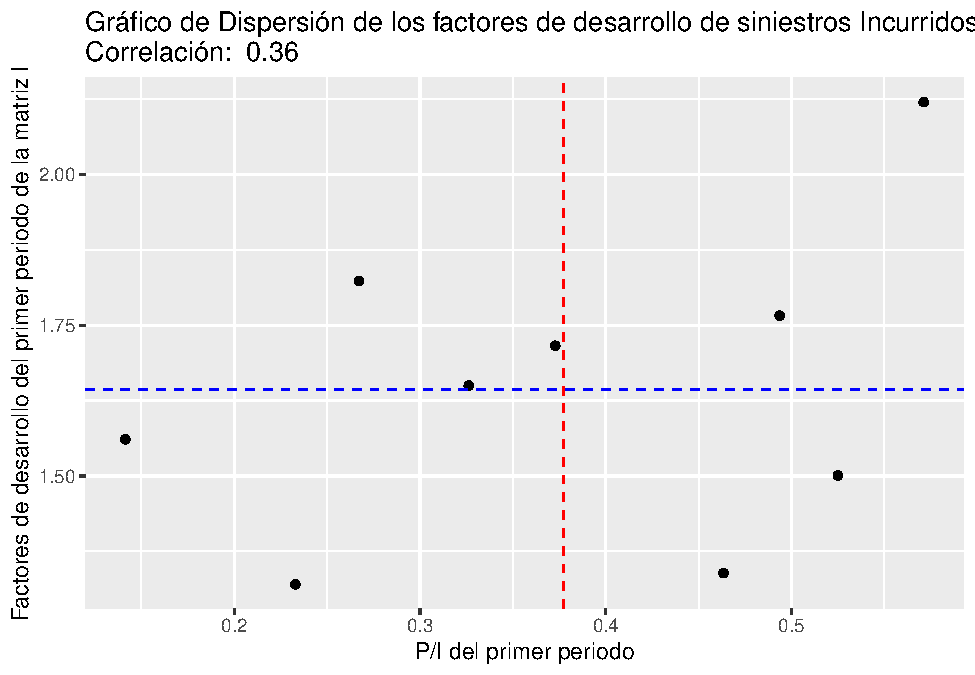
\includegraphics{informe_files/figure-latex/unnamed-chunk-26-1.pdf}

Parece ser que uno de los problemas principales es asumir un factor
igual para todos los años de ocurrencia, dado un período de desarrollo y
se nota que estos factores depende de los ratios \((P/I)\).

También es claro que con el correr de los períodos de desarrollo se
tendrán menos puntos en nuestro gráfico, y los resultados serán menos
consistentes, y además, los factores de desarrollo individuales para
cada año deben ser ajustados tanto para la matriz de pagos acumulados
como la de siniestros incurridos, pero la pregunta es en que medida cada
uno, esto expresa la idea básica para resolver el problema del método
SCL.

Siendo que para cada período de desarrollo se tiene un gráfico de puntos
como el anterior, pero cada vez con menos puntos, la idea es hacer una
regresión lineal en cada caso, y estimar el factor de desarrollo para
cada \((P/I)\), y de esta forma se puede predecir la parte restante de
la matriz. Por ejemplo, para el factor de desarrollo individual
\(q_{1,10}\) que no se tiene valores de la columna siguiente del
triángulo para calcularlo, se puede predecir con la regresión a partir
del valor \((P/I)_{1,10}\)

El método de Munich Chain-Ladder también incorpora los ratios
\((I/P)=1/(P/I)\), y la regresión de los factores de desarrollo de los
pagos acumulados se hace respecto a este ratio.

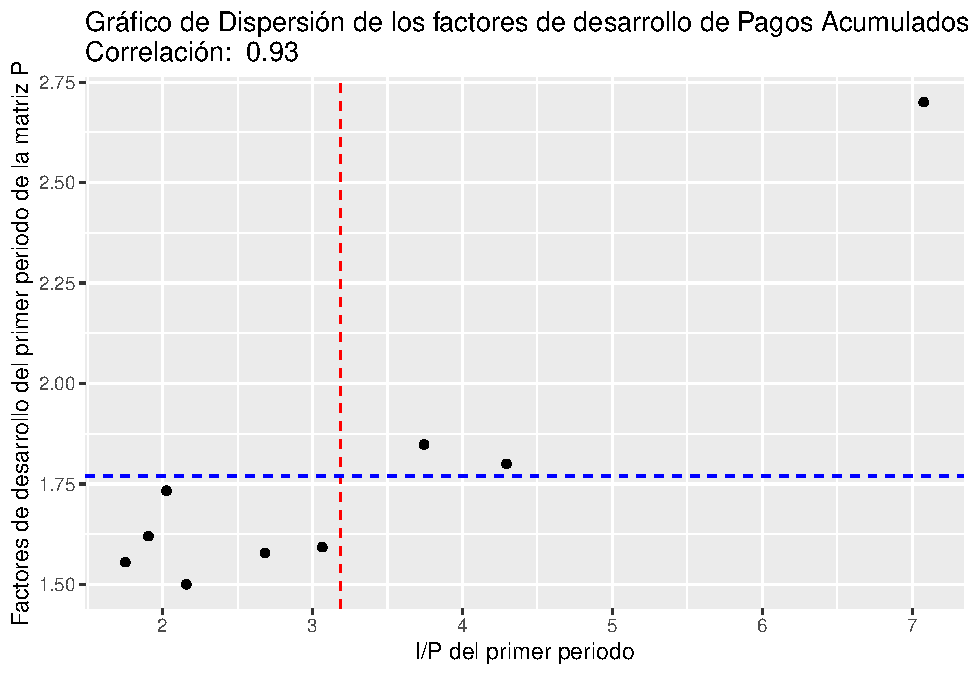
\includegraphics{informe_files/figure-latex/unnamed-chunk-27-1.pdf}

El segundo problema que se puede observar, es que, con el pasar de los
períodos de desarrollo, se tienen menos datos, y las estimaciones son
muy volátiles, incluso algunas veces se pueden obtener regresiones con
el signo incorrecto en el coeficiente. Y por último, a veces no hay una
estructura clara que refleje correlación. O la misma es muy débil.

El método de Munich considera todos los coeficientes de desarrollo
juntos, para todos los años y todos los períodos, y también los ratios
\((P/I)\) y \((I/P)\) teniendo todos los valores estandarizados, es
decir, restando la esperanza y diviendo entre el desvío, obteniendo así
datos con media 0 y desvío 1.

Luego, como los datos están estandarizados, se puede graficar todos los
datos juntos para los factores de desarrollo individuales estandarizados
de los pagos acumulados vs los ratios \((I/P)\) y los factores de
desarrollo individuales estandarizados de los siniestros incurridos vs
los ratios \((P/I)\), luego se puede hacer la regresión con la nube de
puntos que, que ahora tiene más datos, y calcular la estimación de los
factores de desarrollo a partir del modelo lineal. Lo mismo para la
estimación de los factores de desarrollo individuales para los estimar
la parte de la matriz que falta. Todo este método se puede aplicar a
partir de la función `MunichChainLadder' del paquete ChainLadder, a la
que se le debe pasar como argumento los dos triangulos, el de pagos
acumulados y el de siniestros incurridos.

\begin{verbatim}
## MunichChainLadder(Paid = acum, Incurred = tri)
## 
##      Latest Paid Latest Incurred Latest P/I Ratio  Ult. Paid Ult. Incurred
## 1999   4,408,012       5,099,688            0.864  4,408,012     5,099,688
## 2000   3,310,585       4,221,137            0.784  3,516,429     4,285,192
## 2001   2,183,145       5,969,088            0.366  3,938,897     6,078,382
## 2002   5,122,735       8,581,805            0.597  7,450,537     9,075,687
## 2003   2,613,770       7,276,239            0.359  6,336,076     8,419,911
## 2004   2,244,504       5,882,585            0.382  5,950,166     7,535,352
## 2005   4,475,503       9,901,076            0.452 12,013,701    14,652,551
## 2006   5,966,324      12,548,654            0.475 17,995,073    22,028,141
## 2007   4,760,793       9,171,465            0.519 17,172,978    20,825,623
## 2008   4,876,379      10,120,889            0.482 29,364,789    35,705,671
##      Ult. P/I Ratio
## 1999          0.864
## 2000          0.821
## 2001          0.648
## 2002          0.821
## 2003          0.753
## 2004          0.790
## 2005          0.820
## 2006          0.817
## 2007          0.825
## 2008          0.822
## 
## Totals
##              Paid Incurred P/I Ratio
## Latest:   4.0e+07  7.9e+07      0.51
## Ultimate: 1.1e+08  1.3e+08      0.81
\end{verbatim}

Con la función \texttt{plot} pasándole un objeto del tipo
\texttt{MunichChainLadder} genera la siguiente figura con 4 gráficos. El
primero de ellos contiene la estimación de los siniestros pagados e
incurridos ocurridos para cada período mediante el método de Munich
Chain-Ladder, el siguiente gráfico muestra la obtención de los ratios
\((P/I)\) en términos porcentuales obtenidos mediante Munich
Chain-Ladder (MCL), o lo obtenidos si se hacía Chain-Ladder por separado
(Mack), mostrando como así se hubiesen obtenidos ratios por encima de 1
(o por encima de \%100 en términos porcentuales). El gráfico de abajo a
la izquierda, muestra la dispersión de todos los factores centrados y
estandarizados de los pagos acumulados vs los ratios \((I/P)\) con su
respectiva regresión. Y el último gráfico muestra lo mismo pero para los
factores de los siniestros incurridos respceto al ratio \((P/I)\).

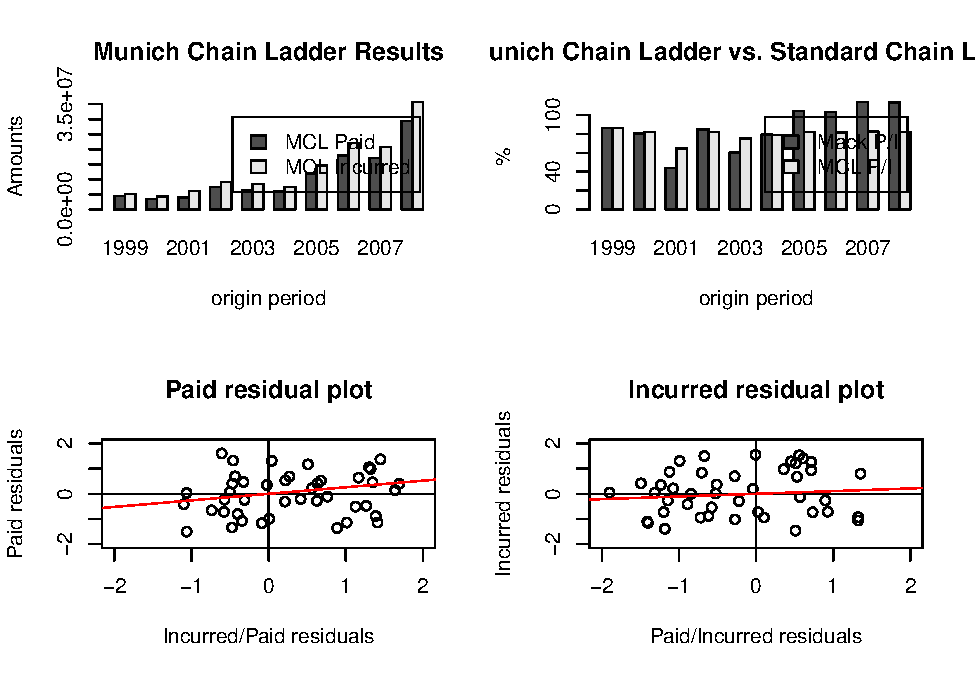
\includegraphics{informe_files/figure-latex/unnamed-chunk-29-1.pdf}

\begin{verbatim}
##      Latest Paid Latest Incurred Latest P/I Ratio Ult. Paid Ult. Incurred
## 1999     4408012         5099688        0.8643690   4408012       5099688
## 2000     3310585         4221137        0.7842876   3516429       4285192
## 2001     2183145         5969088        0.3657418   3938897       6078382
## 2002     5122735         8581805        0.5969298   7450537       9075687
## 2003     2613770         7276239        0.3592200   6336076       8419911
## 2004     2244504         5882585        0.3815507   5950166       7535352
## 2005     4475503         9901076        0.4520219  12013701      14652551
## 2006     5966324        12548654        0.4754553  17995073      22028141
## 2007     4760793         9171465        0.5190875  17172978      20825623
## 2008     4876379        10120889        0.4818133  29364789      35705671
##      Ult. P/I Ratio
## 1999      0.8643690
## 2000      0.8206001
## 2001      0.6480173
## 2002      0.8209337
## 2003      0.7525110
## 2004      0.7896334
## 2005      0.8199051
## 2006      0.8169129
## 2007      0.8246081
## 2008      0.8224125
\end{verbatim}

\begin{verbatim}
##                Paid  Incurred P/I Ratio
## Latest:    39961752  78772626 0.5073051
## Ultimate: 108146657 133706197 0.8088380
\end{verbatim}

Si se estima de esta manera el factor de desarrollo individual para
poder estimar los valores que están enseguida por debajo de la diagonal
invertida, y luego de forma iterativa se completa la matriz, tanto la de
pagos acumulados como la de siniestros incurridos, al final del período,
cuando se evalúen los ratios \((P/I)\) no se obtendrán los valores
mayores a 1 que se obtenían cuando se hacía las dos matrices por
separado.

\%knitr::include\_graphics(``imagenes/condicional\_normal.png'')

\%\protect\hyperlink{bib}{Nadaraya-Watson}

\newpage

\hypertarget{bib}{%
\section*{Bibliografía}\label{bib}}
\addcontentsline{toc}{section}{Bibliografía}

\hypertarget{refs}{}
\begin{CSLReferences}{1}{0}
\leavevmode\vadjust pre{\hypertarget{ref-chain}{}}%
Gesmann, Markus, Daniel Murphy, Yanwei (Wayne) Zhang, Alessandro
Carrato, Mario Wuthrich, Fabio Concina, y Eric Dal Moro. 2023.
\emph{ChainLadder: Statistical Methods and Models for Claims Reserving
in General Insurance}.
\url{https://CRAN.R-project.org/package=ChainLadder}.

\end{CSLReferences}

\hypertarget{material-adicional}{%
\section*{Material adicional}\label{material-adicional}}
\addcontentsline{toc}{section}{Material adicional}

La entrega del informe viene acompañado de 2 scripts, que contienen la
implementación de cada método presentado junto con las aplicaciones
realizadas:

\begin{itemize}
\item
  \texttt{quantile\_regression\_by\_huang-nguyen.R}
\item
  \texttt{quantile\_regression\_by\_yu-jones.R}
\end{itemize}

\end{document}
